\documentclass[a4paper,12pt,titlepage]{article}

\usepackage[latin1]{inputenc}
\usepackage{amsmath}
\usepackage[english]{babel}
\usepackage[T1]{fontenc}
\usepackage{graphicx}
\usepackage{xcolor}
\usepackage{listings}

\author{Jean-Denis Lesage, Benjamin Petit, Bruno Raffin, Antoine Vanel}
\title{FlowVR-Render Tutorial}
\date{12/11/2008}

\newcommand{\more}[1]{\label{A VOIR !!!!} \fbox{A VOIR}\ {\small{ \em #1}}}
\newcommand{\nomore}[1]{}
%\newcommand{\example}[1]{\Huge Example : #1}

\lstset{showstringspaces=false,frame=trbL,columns=flexible,fontadjust=true}
\lstdefinestyle{bash}{language=bash}
\lstdefinestyle{Perl}{language=Perl}
\lstdefinestyle{C++}{language=C++}
\lstdefinestyle{DTD}{language=XML}
\lstdefinestyle{XML}{language=XML,usekeywordsintag=false,markfirstintag=true}
\lstnewenvironment{codeflowvr}{}{}
\lstnewenvironment{codeflowvr_bash}{\lstset{style=bash}}{}
\lstnewenvironment{codeflowvr_perl}{\lstset{style=Perl}}{}
\lstnewenvironment{codeflowvr_cpp}{\lstset{style=C++}}{}
\lstnewenvironment{codeflowvr_dtd}{\lstset{style=DTD}}{}
\lstnewenvironment{codeflowvr_xml}{\lstset{style=XML}}{}

\begin{document}
\maketitle
\section{Introduction}
\more{Objectif � �crire}

\section{FlowVR-app Network}
\subsection{Tutorial Component}
This composite component contains 2 main components:
\begin{itemize}
    \item ViewerGroup: A container with all viewers. A viewer creates FlowVR-Render primitives.
    \item Renderer: A high-level component rendering all the primitives coming from the viewers. Communication schemes and swaplock are included in this component. See FlowVR-Renderer Usage Example for more details.
\end{itemize}

\begin{figure}[ht]
    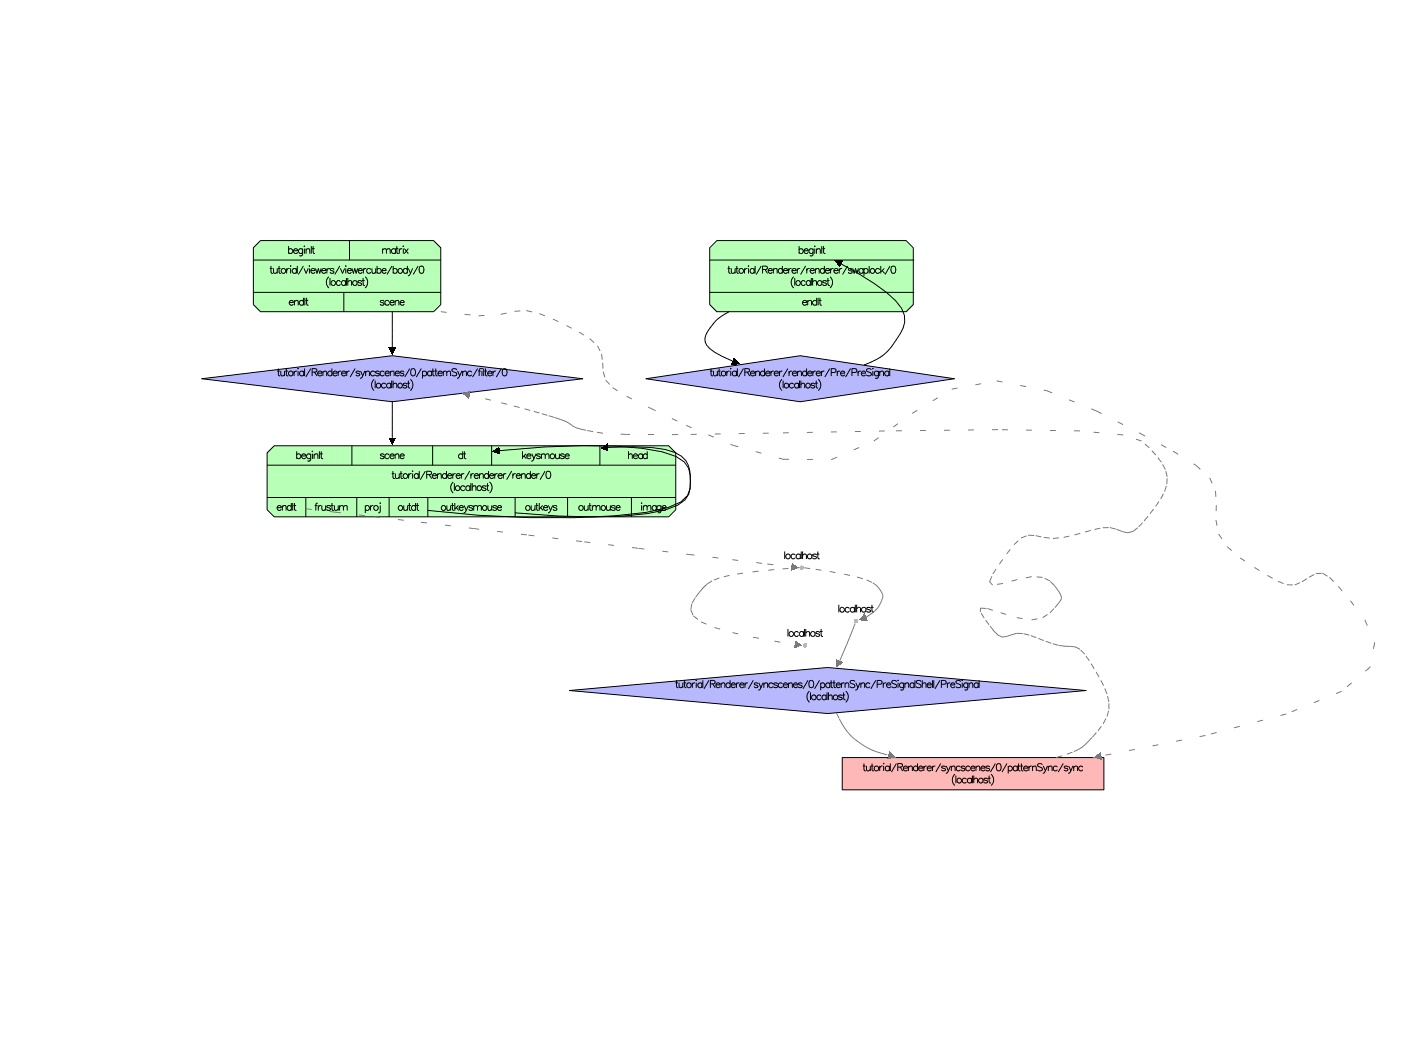
\includegraphics[width=\textwidth]{figures/network.jpg}
    \caption{Tutorial Network}
\end{figure}

\subsection{Create a Viewer}

A Viewer is a specific FlowVR Module with an output port (often named \textit{scene}) sending scene primitives. FlowVR-render extends the FlowVR-app standard library to provide a ModuleViewer class that eases the description of new viewer. This class extends the FlowVR-app Module class to add a \textit{scene} port. \par

If your viewer doesn't need other new ports, you can use directly the ModuleViewer class to describe your viewer and to create a MetaModule that launches the process associated to your viewer. \par

The MetaModule describing the first viewer of this tutorial (the viewer cube, refer to section \ref{cube} for more details) is an example. The name of the executable is set using the constructor as for standard metamodule.\par

\begin{codeflowvr_cpp}
    // The goal of this component is to encapsulate viewer component and add a command line to launch it
    // ModuleViewer is a generic class with the common interface of viewer components. Use it if your viewer has only a scene and a matrix ports.
    class MetaModuleViewerCube : public MetaModuleFlowvrRunSSHSingleton<ModuleViewer>
    {
    public :
    MetaModuleViewerCube(const std::string& id_ ) : MetaModuleFlowvrRunSSHSingleton<ModuleViewer>(id_, CmdLine("viewercube") )
    {
    setInfo("Metamodule launching viewer cube  module");
    };

    //Mandatory virtual destructor
    virtual ~MetaModuleViewerCube(){};

    // Mandatory create  method
    virtual Component* create() const { return new MetaModuleViewerCube(getId());};
    };
\end{codeflowvr_cpp} \par

\subsection{ViewersGroup Component}

In this tutorial, we use this composite component (ViewersGroup) as a container for all viewers. This component has only an output port \textit{scenes} gathering primitives from all viewers. These primitives will be sent to the Renderer. The Renderer component will then merge and render all the primitives.\par 

To add a new viewer in this container, we only need to add the MetaModule of the viewer and link its \texttt{scene} port with the \texttt{scenes} port of the ViewersGroup which will be later linked to the \texttt{scene} port of the Renderer. For instance, in the ViewersGroup::execute() method, these two instructions add and link the MetaModuleViewerCube:

\begin{codeflowvr_cpp}
    Component* viewercube = addObject<MetaModuleViewerCube>("viewercube");
    link(viewercube->getPort("scene"), getPort("scenes"));
\end{codeflowvr_cpp} \par

The parameter \texttt{example} enables to select which example must be executed. That is the possible values:
\begin{enumerate}
    \item Cube (Section \ref{cube})
    \item Sphere (Section \ref{sphere})
    \item Obj (Section \ref{obj})
    \item Cube + Sphere + Obj (Section \ref{blend})
    \item Custom Shader (Section \ref{shaders})
    \item Texturing a Quad (Section \ref{texture})
    \item Cube + Billboard with different scales (Section \ref{scale})
    \item Ressource Sharing (Section \ref{ressources})
\end{enumerate}

\section{Cube Viewer} 
\label{cube}

\subsection{Usage}

\texttt{flowvr -L Tutorial -P tutorial:example=1 -x -s -l}

\begin{figure}[ht]
    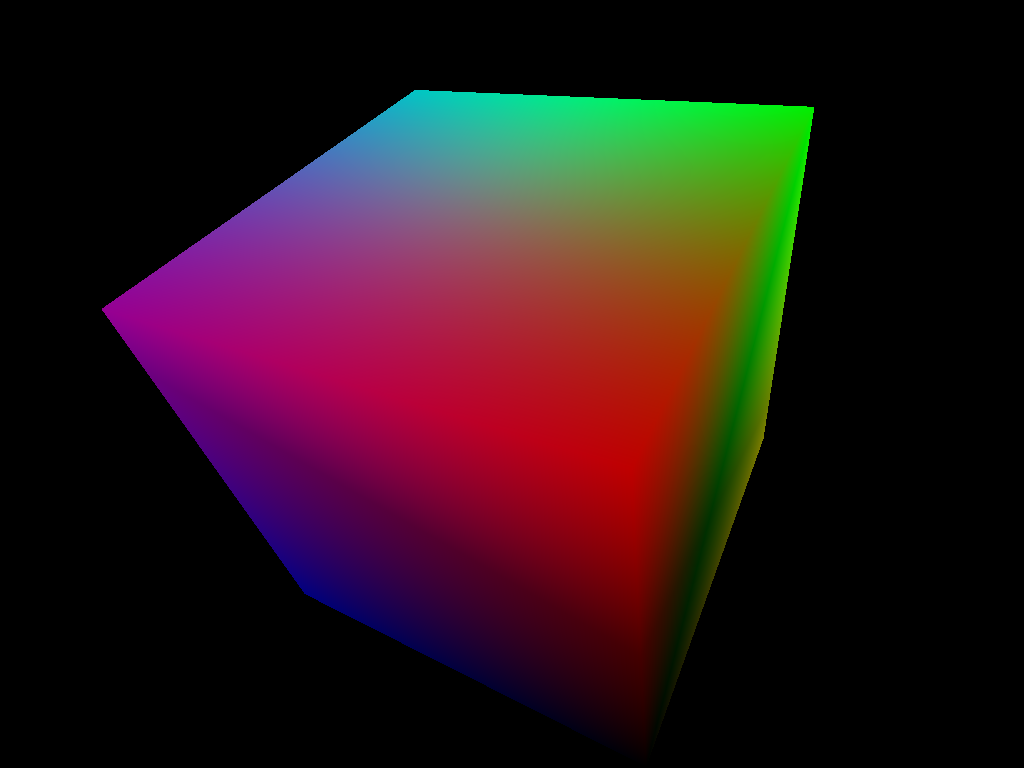
\includegraphics[width=\textwidth]{figures/cube.png}
    \caption{Primitive Cube}
\end{figure}

\subsection{Viewer Source Code Explanation}

First, the interface of the module must be declared to the daemon as a standard FlowVR module. The port that will send the scene is a specific type of port (Type SceneOutputPort instead of OutputPort)

\begin{codeflowvr_cpp}
    int main(int argc, char** argv)
    
    	// Declare a FlowVR Render output port to send our scene description.
    	SceneOutputPort pOut("scene");

    	// Initialize FlowVR
    	std::vector<flowvr::Port*> ports;
    	ports.push_back(&pOut);
    	flowvr::ModuleAPI* module = flowvr::initModule(ports);

    	if (module == NULL)
    		return 1;
\end{codeflowvr_cpp} \par

A specific class defines message with the scene primitives:
\begin{codeflowvr_cpp}
    flowvr::render::ChunkRenderWriter scene;
\end{codeflowvr_cpp}  \par

At the first iteration, we have to declare the IDs of objects involved in the scene. There are two kind of objects:
\begin{itemize}
    \item Primitives
    \item Resources
\end{itemize}

A primitives contains references (ID) to several resources. A primitive should have at least these two ressources:
\begin{itemize}
	\item a vertex buffer
	\item an index buffer
\end{itemize}

A resource could be shared between different primitives.\par

In this example, we have one primitive with a vertex buffer and an index buffer. The following code will create their ID:

\begin{codeflowvr_cpp}
    // Reserve IDs for all our primitives and resources
    ID idPrim = module->generateID(); // Id of the primitive
    ID idVB = module->generateID(); // Id of the Vertex Buffer
    ID idIB = module->generateID(); // Id of the Index Buffer
\end{codeflowvr_cpp}  \par

Then, we fill the ressources. First, we need to reserve necessary space in the FlowVR message.

\begin{codeflowvr_cpp}
    // Create vertex+index buffers for a cube
    // We use three vertex buffers (position, normal and color). This array provides the number of vertex buffers and their types
    int vertexBufferTypes[3] = {Type::Vec3f, Type::Vec3f, Type::Vec3f};
    // Create the vertex buffers (8 points and 2 buffers)
    ChunkVertexBuffer* vb = scene.addVertexBuffer(idVB, 8, 3, vertexBufferTypes);
    // Create the index buffer (12 triangles = 12*3 values of type Byte)
    int indexBufferType = Type::Byte;
    ChunkIndexBuffer* ib = scene.addIndexBuffer(idIB, 12*3, indexBufferType, ChunkIndexBuffer::Triangle);
\end{codeflowvr_cpp} \par

After this reservation, the vertex buffer in the FlowVR message will have the following structure (Fig \ref{vbuffer})
\begin{figure}
    %\includegraphics[width=\textwidth]{figures/vbuffer.png}
    \caption{Vertex Buffer Structure}
    \label{vbuffer}
\end{figure}

The data can be set directly on this data section:

\begin{codeflowvr_cpp}
    // Fill vertex and index buffers 
    Vec3f* vdata = (Vec3f*) vb->data();
    // Positions = vdata[3*i] values
    // Normal = vdata[3*i + 1] values
    // Colors = vdata[3*i + 2] values
    vdata[3*0] = Vec3f(-1.0, -1.0, -1.0); 
    vdata[3*1] = Vec3f(1.0, -1.0, -1.0); 
    vdata[3*2] = Vec3f(1.0, 1.0, -1.0); 
    vdata[3*3] = Vec3f(-1.0, 1.0, -1.0); 
    vdata[3*4] = Vec3f(-1.0, -1.0, 1.0); 
    vdata[3*5] = Vec3f(1.0, -1.0, 1.0); 
    vdata[3*6] = Vec3f(1.0, 1.0, 1.0); 
    vdata[3*7] = Vec3f(-1.0, 1.0, 1.0); 

    // Normals = Positions for this example
    for(unsigned int i = 0; i != 8; ++i)
    {
    	vdata[3*i +1] = vdata[3*i];
    	vdata[3*i +1].normalize();
    }

    // A different color for each vertices
    for(unsigned int i = 0; i != 8; ++i)
    {
    	vdata[3*i+2] = Vec3f((float)(i&1), (float)((i>>1)&1), (float)((i>>2)&1));
    }
\end{codeflowvr_cpp} \par

Then we set the index buffer:

\begin{codeflowvr_cpp}

    // Index buffer. We set values of the 12 triangles
    Vec<3,char>* idata = (Vec<3,char>*) ib->data();
    idata[0] = Vec<3,char>(0, 2, 1); 
    idata[1] = Vec<3,char>(0, 3, 2); 
    idata[2] = Vec<3,char>(0, 1, 4); 
    idata[3] = Vec<3,char>(1, 5, 4); 
    idata[4] = Vec<3,char>(3, 7, 0); 
    idata[5] = Vec<3,char>(0, 7, 4); 
    idata[6] = Vec<3,char>(4, 6, 5); 
    idata[7] = Vec<3,char>(4, 7, 6); 
    idata[8] = Vec<3,char>(1, 5, 2); 
    idata[9] = Vec<3,char>(2, 5, 6); 
    idata[10] = Vec<3,char>(2, 3, 6); 
    idata[11] = Vec<3,char>(6, 3, 7); 
\end{codeflowvr_cpp} \par

Now, the primitive can be created:

\begin{codeflowvr_cpp}
    // Create new primitive
    scene.addPrimitive(idPrim, "Cube");
\end{codeflowvr_cpp} \par

And we link ressources using the \texttt{addParamID} method. First, we link the vertex buffer resource. Two steps compose this link:

\begin{enumerate}
    \item Enumeration of data included in the buffer (here position, normal and color)
    \item The place of this data in the buffer (following the structure presented in figure \ref{vbuffer})
\end{enumerate}

\begin{codeflowvr_cpp}
    // Link vertex buffer idVB to primitive idPrim
    // Position, normal and color are given by vertexbuffer idVB
    scene.addParamID(idPrim, ChunkPrimParam::VBUFFER_ID, "position", idVB);
    scene.addParamID(idPrim, ChunkPrimParam::VBUFFER_ID,"normal",idVB);
    scene.addParamID(idPrim, ChunkPrimParam::VBUFFER_ID,"color0",idVB);
    // Position is 1rst value for each point. Its offset is 0 (default case)
    // Normal is the 2nd value for each point. Its offset is 1
    scene.addParamID(idPrim, ChunkPrimParam::VBUFFER_NUMDATA,"normal",1);
    // Color is the 3rd value for each point. Its offset is 2
    scene.addParamID(idPrim, ChunkPrimParam::VBUFFER_NUMDATA,"color0",2);
\end{codeflowvr_cpp} \par 

The index buffer is linked to the primitive:

\begin{codeflowvr_cpp} 
    // Link index buffer idIB to primitivie idPrim
    scene.addParamID(idPrim, ChunkPrimParam::IBUFFER_ID, "", idIB);
\end{codeflowvr_cpp} \par

Global parameter as the light vector for the shading or projection matrices can be associated to a primitive using the \texttt{addParam} or \texttt{addParamEnum} methods. 

\begin{codeflowvr_cpp}
    // Set shaders parameters
    // Note: We do not redefine the shader for this primitive so these
    // parameters correspond to the default shaders.
    // See data/shaders/default_v.cg and data/shaders/default_p.cg
    // See also shaders examples in this tutorial
    scene.addParamEnum(idPrim, ChunkPrimParam::PARAMVSHADER, "ModelViewProj", ChunkPrimParam::ModelViewProjection);
    scene.addParamEnum(idPrim, ChunkPrimParam::PARAMVSHADER, "ModelView", ChunkPrimParam::ModelView);
    scene.addParamEnum(idPrim, ChunkPrimParam::PARAMVSHADER, "ModelViewIT", ChunkPrimParam::ModelView_InvTrans);
    Vec3f light(1,3,2); light.normalize();
    scene.addParam(idPrim, ChunkPrimParam::PARAMPSHADER, "lightdir", light);
\end{codeflowvr_cpp} \par 

A specific example is dedicated to these methods \texttt{addParamID}, \texttt{addParam} and \texttt{addParamEnum} and shaders customization. Refer to the section \ref{shaders} for more details. \par

At least, we can write the main FlowVR loop. Here, the scene is static, so we just send the message at each iteration. 

\begin{codeflowvr_cpp}

    // Main FlowVR loop. Contains the animations of the scene
    while (module->wait())
    {
    	// Update scene
    	// Nothing in this simple example...

    	// Send message
    	scene.put(&pOut);
    	sleep(1);	//To avoid overflow
    }

    module->close();

    return 0;

\end{codeflowvr_cpp} \par

\section{Sphere Viewer}
\label{sphere}

\section{Obj Model Viewer}
\label{obj}
\subsection{Usage}

\texttt{flowvr -L Tutorial -P``tutorial:example=3 tutorial:OBJFILE=bunny.obj'' -x -s -l}

\subsection{Viewer Explanation}
This viewer reads a 3D model with the wavefront object format (.obj) and displays it using FlowVR-Render primitives. The parameter OBJFILE of the MetaModule is set to obj file path. This metamodule can be used to populate your scene using directly obj files.\par 

\section{Blend Viewers}
\label{blend}

\section{FlowVR-Renderer Usage (display walls, options, special keys ...)}

\section{Shaders parameters}
\label{shaders}

\section{Texturing}
\label{texture}

\subsection{Usage}

\texttt{flowvr -L Tutorial -P tutorial:example=2 tutorial:textureFileName=exampleTexture.jpg -x -s -l}

You can try another image filename instead of exampleTexture.jpg

\begin{figure}[ht]
    %\includegraphics[width=\textwidth]{figures/texture.png}
    \caption{Primitive Quad + texture}
\end{figure}

\subsection{Viewer Source Code Explanation}

\section{How Scale Primitives}
\label{scale}

%\section{Tracking: ID\_CAMERA}	

\section{Ressources Sharing}
\label{ressources}

\end{document}
